\documentclass[border=5pt]{standalone}
\usepackage[T1]{fontenc}
\usepackage{lmodern}
\usepackage{pgfplots}
\usepgfplotslibrary{groupplots}
\pgfplotsset{compat=1.18}
\begin{document}
\sffamily
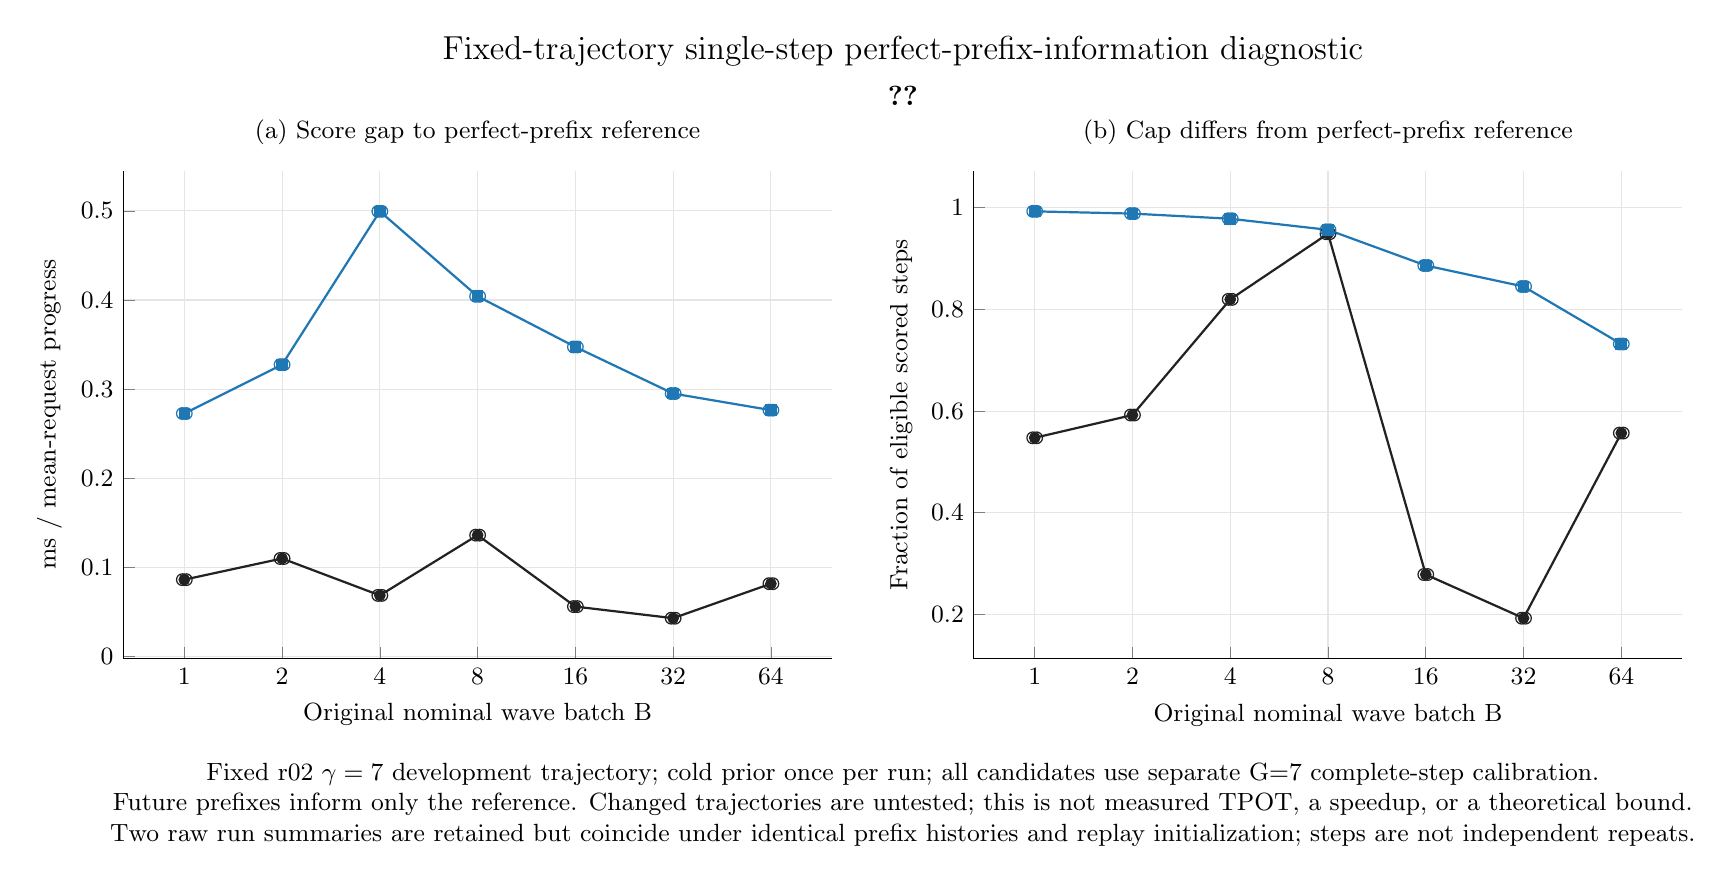
\begin{tikzpicture}
\definecolor{series0}{HTML}{222222}
\definecolor{series1}{HTML}{1f77b4}
\definecolor{series2}{HTML}{ff7f0e}
\definecolor{series3}{HTML}{2ca02c}
\definecolor{series4}{HTML}{d62728}
\definecolor{series5}{HTML}{9467bd}
\definecolor{series6}{HTML}{8c564b}
\definecolor{series7}{HTML}{e377c2}
\begin{groupplot}[group style={group size=2 by 1,horizontal sep=1.8cm},width=9.0cm,height=6.2cm,scale only axis,grid=major,grid style={gray!20},axis lines*=left,tick label style={font=\small},label style={font=\small},title style={font=\small},unbounded coords=jump]
\nextgroupplot[title={(a) Score gap to perfect-prefix reference},xlabel={Original nominal wave batch B},ylabel={ms / mean-request progress},xtick={1,2,4,8,16,32,64},xticklabels={1,2,4,8,16,32,64},xmode=log,log basis x=2,minor x tick num=0,scaled y ticks=false,yticklabel style={/pgf/number format/fixed,/pgf/number format/precision=2},legend columns=2,legend to name=sharedlegend,legend style={draw=none,font=\small,/tikz/every even column/.append style={column sep=8pt}}]
\addplot+[color=series0,mark=*,mark size=1.7pt,mark options={fill=series0,draw=series0},line width=0.8pt] coordinates {(1,0.0860922026131) (2,0.109864291239) (4,0.068425505121) (8,0.136072782668) (16,0.0558673044869) (32,0.0428446482607) (64,0.0815603563718)};
\addlegendentry{Replayed pre-step cap}
\addplot+[only marks,forget plot,color=series0,mark=o,mark size=2.1pt,mark options={fill=white,line width=0.45pt}] coordinates {(0.986097544263,0.0860922026131) (1.01409845894,0.0860922026131) (1.97219508853,0.109864291239) (2.02819691788,0.109864291239) (3.94439017705,0.068425505121) (4.05639383575,0.068425505121) (7.8887803541,0.136072782668) (8.11278767151,0.136072782668) (15.7775607082,0.0558673044869) (16.225575343,0.0558673044869) (31.5551214164,0.0428446482607) (32.451150686,0.0428446482607) (63.1102428328,0.0815603563718) (64.9023013721,0.0815603563718)};
\addplot+[color=series1,mark=square*,mark size=1.7pt,mark options={fill=series1,draw=series1},line width=0.8pt] coordinates {(1,0.272564432465) (2,0.327395418601) (4,0.499476334883) (8,0.404130819142) (16,0.347284030305) (32,0.294987585739) (64,0.276364700819)};
\addlegendentry{Recorded cap7}
\addplot+[only marks,forget plot,color=series1,mark=o,mark size=2.1pt,mark options={fill=white,line width=0.45pt}] coordinates {(0.986097544263,0.272564432465) (1.01409845894,0.272564432465) (1.97219508853,0.327395418601) (2.02819691788,0.327395418601) (3.94439017705,0.499476334883) (4.05639383575,0.499476334883) (7.8887803541,0.404130819142) (8.11278767151,0.404130819142) (15.7775607082,0.347284030305) (16.225575343,0.347284030305) (31.5551214164,0.294987585739) (32.451150686,0.294987585739) (63.1102428328,0.276364700819) (64.9023013721,0.276364700819)};
\nextgroupplot[title={(b) Cap differs from perfect-prefix reference},xlabel={Original nominal wave batch B},ylabel={Fraction of eligible scored steps},xtick={1,2,4,8,16,32,64},xticklabels={1,2,4,8,16,32,64},xmode=log,log basis x=2,minor x tick num=0,scaled y ticks=false,yticklabel style={/pgf/number format/fixed,/pgf/number format/precision=2}]
\addplot+[color=series0,mark=*,mark size=1.7pt,mark options={fill=series0,draw=series0},line width=0.8pt] coordinates {(1,0.547389615993) (2,0.59219858156) (4,0.819751753913) (8,0.949023861171) (16,0.278396436526) (32,0.192488262911) (64,0.556701030928)};
\addplot+[only marks,forget plot,color=series0,mark=o,mark size=2.1pt,mark options={fill=white,line width=0.45pt}] coordinates {(0.986097544263,0.547389615993) (1.01409845894,0.547389615993) (1.97219508853,0.59219858156) (2.02819691788,0.59219858156) (3.94439017705,0.819751753913) (4.05639383575,0.819751753913) (7.8887803541,0.949023861171) (8.11278767151,0.949023861171) (15.7775607082,0.278396436526) (16.225575343,0.278396436526) (31.5551214164,0.192488262911) (32.451150686,0.192488262911) (63.1102428328,0.556701030928) (64.9023013721,0.556701030928)};
\addplot+[color=series1,mark=square*,mark size=1.7pt,mark options={fill=series1,draw=series1},line width=0.8pt] coordinates {(1,0.992952682295) (2,0.988543371522) (4,0.978413383702) (8,0.956616052061) (16,0.886414253898) (32,0.845070422535) (64,0.731958762887)};
\addplot+[only marks,forget plot,color=series1,mark=o,mark size=2.1pt,mark options={fill=white,line width=0.45pt}] coordinates {(0.986097544263,0.992952682295) (1.01409845894,0.992952682295) (1.97219508853,0.988543371522) (2.02819691788,0.988543371522) (3.94439017705,0.978413383702) (4.05639383575,0.978413383702) (7.8887803541,0.956616052061) (8.11278767151,0.956616052061) (15.7775607082,0.886414253898) (16.225575343,0.886414253898) (31.5551214164,0.845070422535) (32.451150686,0.845070422535) (63.1102428328,0.731958762887) (64.9023013721,0.731958762887)};
\end{groupplot}
\path (group c1r1.north west) -- node[above=1.2cm,font=\large] {Fixed-trajectory single-step perfect-prefix-information diagnostic} (group c2r1.north east);
\path (group c1r1.north west) -- node[above=0.7cm] {\ref{sharedlegend}} (group c2r1.north east);
\path (group c1r1.south west) -- node[below=1.2cm,align=center,font=\small] {Fixed r02 $\gamma=7$ development trajectory; cold prior once per run; all candidates use separate G=7 complete-step calibration.\\Future prefixes inform only the reference. Changed trajectories are untested; this is not measured TPOT, a speedup, or a theoretical bound.\\Two raw run summaries are retained but coincide under identical prefix histories and replay initialization; steps are not independent repeats.} (group c2r1.south east);
\end{tikzpicture}
\end{document}
